%!TEX root = main.tex
\section{Analysis}
\label{sec:analysis}

We now analyze further our network, and in particular explore the robustness of our network to departures from the assumptions that were made in sec.~\ref{sec:proposed_method}. 

\subsection{Camera calibration error}

To constrain the set of possible lighting directions (sec.~\ref{sec:analemma}), we made the assumption that the camera is pointing north. We analyzed the impact on reconstruction performance when this hypothesis is infringed by rotating the real environment maps used to render the evaluation dataset (sec.~\ref{sec:evaluation_dataset}), and show the results of this experiment in fig.~\ref{fig:calibration_error_performance}. The slight improvement around $5\degr$ west calibration error is due to the timestamps of our real lighting dataset that are not perfectly aligned with the neural network expected timestamps. We observe that the median reconstruction error increases of approximately $5\degr$ per $10\degr$ error on camera calibration, showing that the network has some built-in robustness to these errors. 


\begin{figure}[!t]
\centering
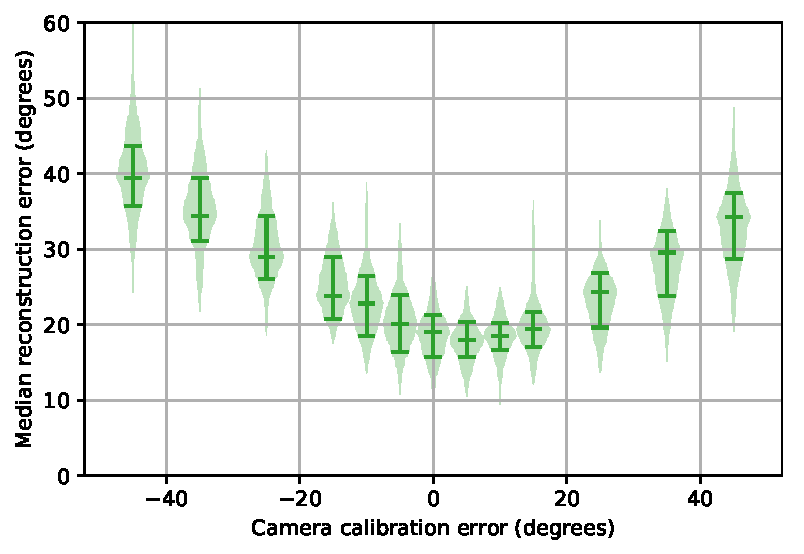
\includegraphics[width=0.7\linewidth]{figures/analysis/performance_calibration_error.pdf}
\caption[Surface reconstruction performance in function of camera calibration error]{Median normal estimation error as box-percentile plots (see fig.~\ref{fig:results-quantitative}) in function of the camera deviation from north in degrees on our real lighting dataset. Positive means camera going toward west, negative means camera going toward east. }
\label{fig:calibration_error_performance}
\end{figure}


\subsection{Number of images}
\label{sec:ablation_study}

We now study the normal estimation performance in function of the number of inputs $T$ to the CNN (see sec.~\ref{sec:architecture}). Results ranging from a single input image ($T=1$, effectively performing shape-from-shading) to $T=16$ input images all uniformly taken from 9:00 to 16:00 are shown in fig.~\ref{fig:number_of_inputs}. We observe an rapid improvement in performance from one to three images, which is coherent with Photometric Stereo theory~\cite{woodham-opteng-80}. Performance continues to increase until $T=8$, probably because added constraints improves robustness to noise and non-diffuse materials. Interestingly, the normal estimation error starts to increase slightly with $T > 8$. This could be due to an increase in the number of parameters to train in our model (the output tensor after concatenation is of dimension $14 \times 14 \times 32T$, thereby increasing the number of parameters in the second convolutional layer), making the model harder to train.

% It is interesting to note the performance of the single image case, where the model obtains better than 24 degree median reconstruction error for half the renders, which is still quite competitive.


\begin{figure}[!t]
\centering
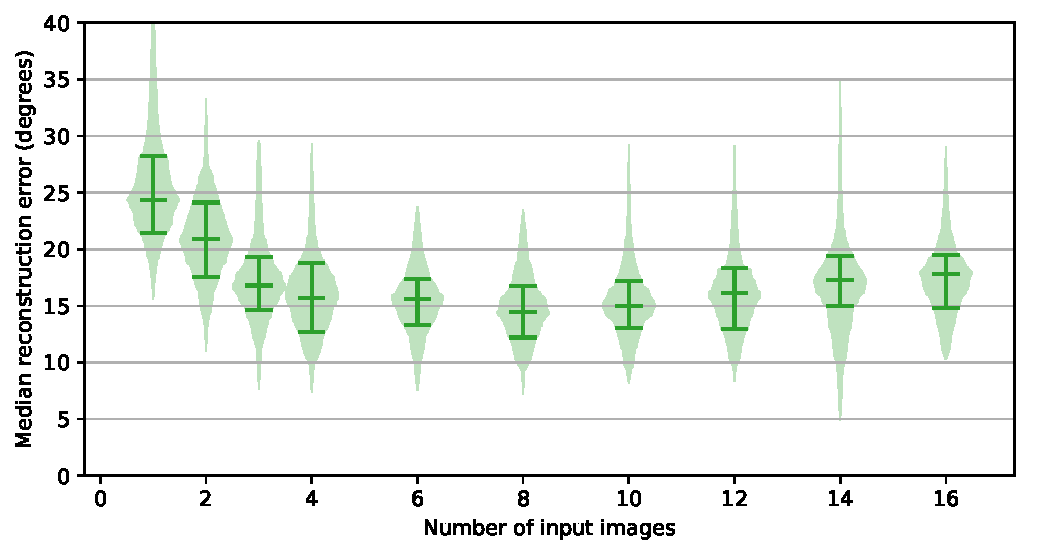
\includegraphics[width=0.75\linewidth]{figures/analysis/input_ablation.pdf}
\caption[Ablation study: surface reconstruction performance in function of the number of input images]{Median normal estimation error as box-percentile plots~\cite{esty-jss-03} (see fig.~\ref{fig:results-quantitative}) on our evaluation dataset as a function of $T$, the number of input images.}
\label{fig:number_of_inputs}
\end{figure}


\subsection{Feature analysis}

We use SmoothGrad~\cite{smilkov-arxiv-17} to visualize the regions of the image that have a larger impact on normal estimation. Since the network operates on patches and not entire images, we use the same linear blending strategy as in sec.~\ref{sec:training_dataset}, and report qualitative results in fig.~\ref{fig:smoothgrad}. We observe how the neural network tends to ignore darker regions and focuses on brighter alternatives in other images when available. This result suggests that the network learns to avoid shadowed areas, where, indeed, the photometric cue is not reliable due to low signal-to-noise ratio and to occlusion of the main light source.


\begin{figure}[!t]
\centering
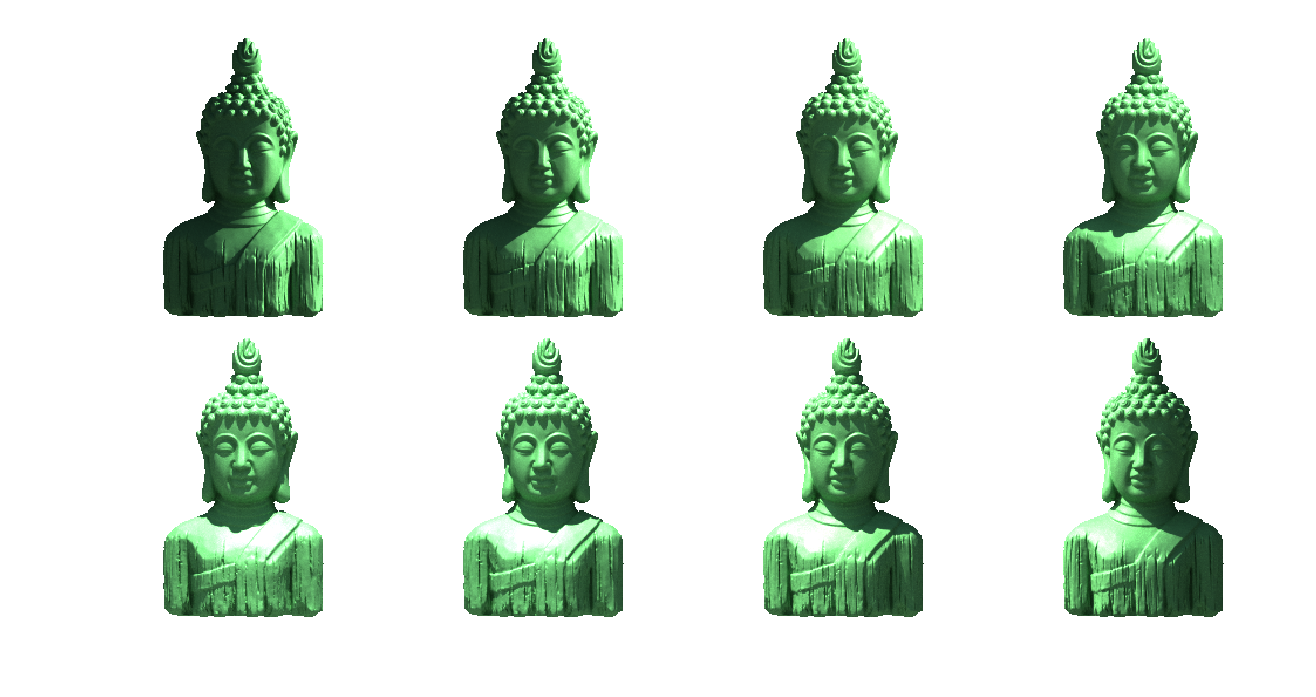
\includegraphics[width=0.49\linewidth]{figures/analysis/smoothgrad_inputs.png}
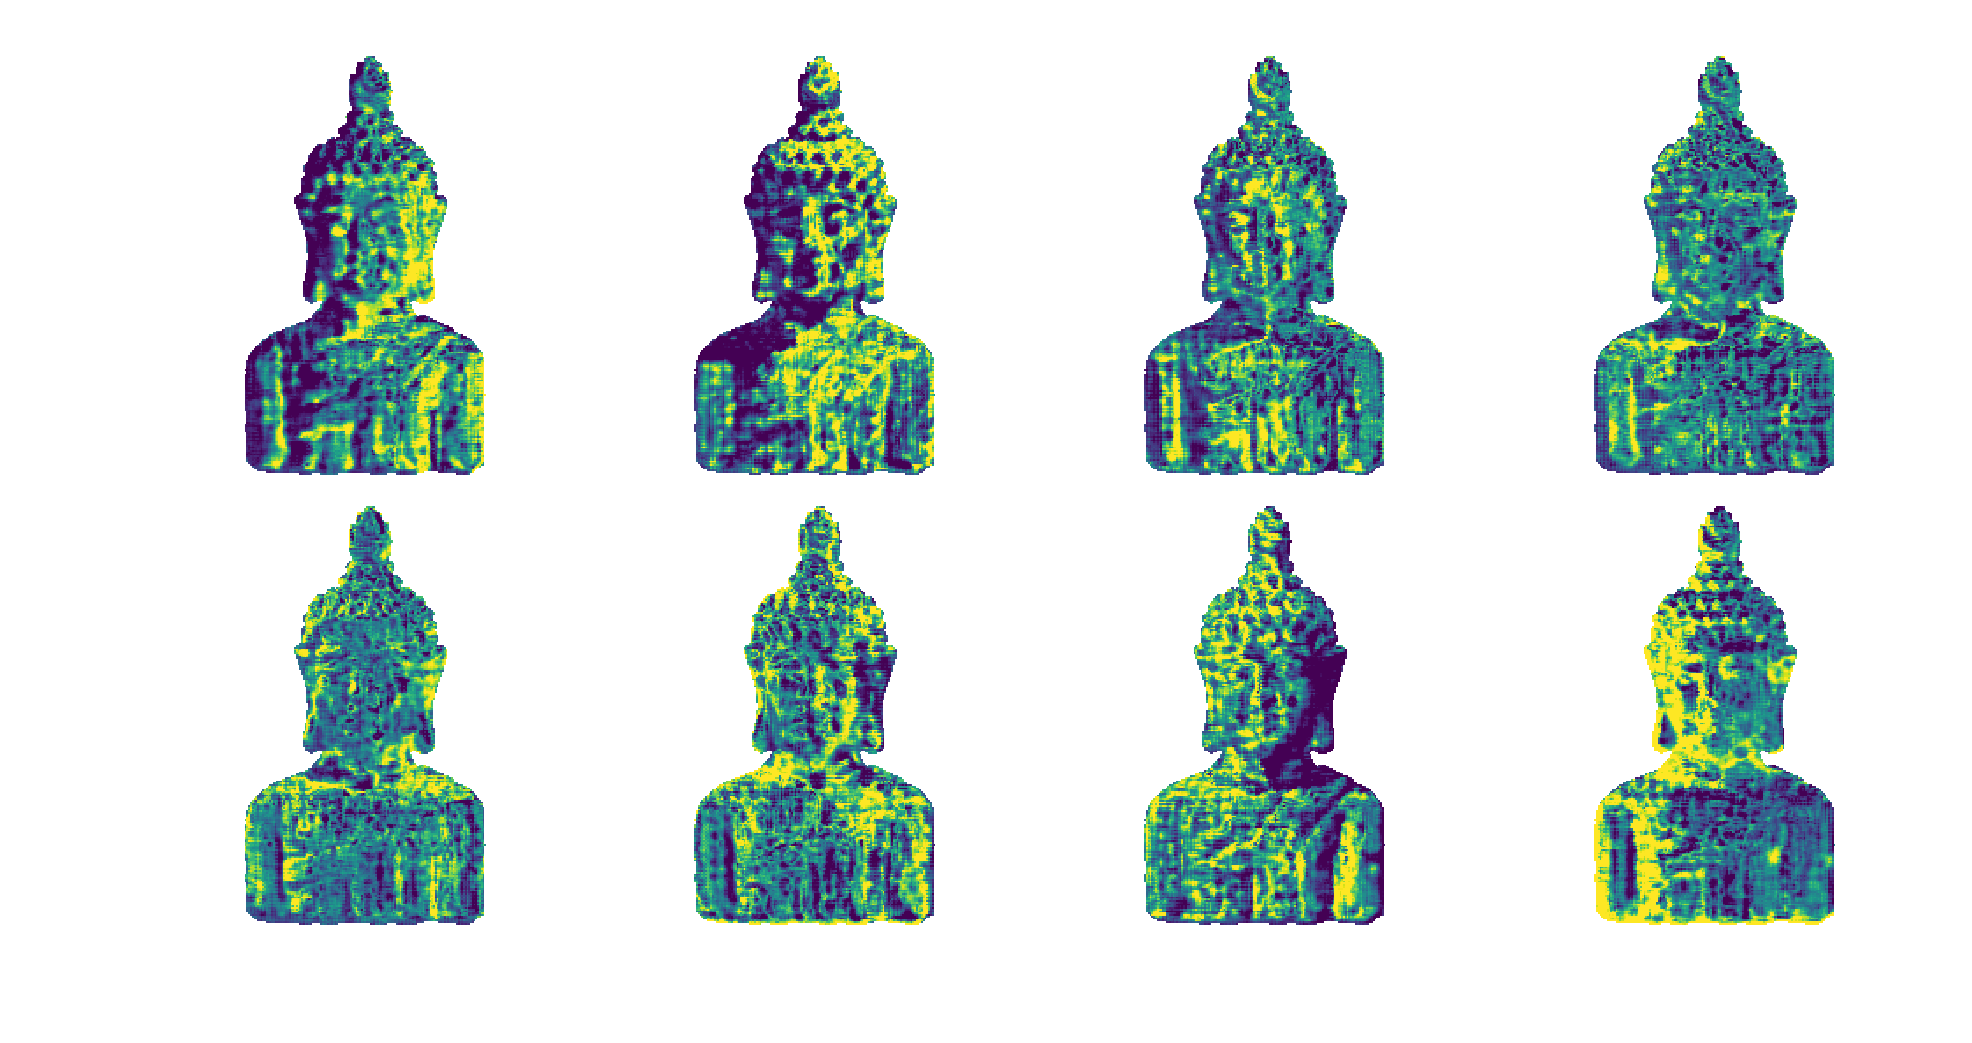
\includegraphics[width=0.49\linewidth]{figures/analysis/smoothgrad.png} \\
\vspace{-1em}
\hspace*{-0.1cm}\begin{tabular*}{\linewidth}{c@{\extracolsep{\fill}}c}
 & 
\includegraphics[width=0.46\linewidth]{figures/analysis/colorbar_smoothgrad_horizontal.pdf}
\end{tabular*} \\
\vspace{-0.7em}
\hspace*{0.4cm}\begin{tabular*}{0.53\linewidth}{c@{\extracolsep{\fill}}c}
(a) & (b)
\end{tabular*} \\
\caption[CNN focus analysis]{Back-propagating the gradient through our network using SmoothGrad~\cite{smilkov-arxiv-17} on the input images shown in (a) generates a map of the pixels that affects the most the normal estimation (b). Notice how the regions in shadow have generally less influence (blue) than regions in direct sunlight (yellow).}
\label{fig:smoothgrad}
\end{figure}

